\documentclass{article}
\usepackage{graphicx} % Required for inserting images
\usepackage{amsmath, amssymb}
\usepackage{mathtools}

\newenvironment{problem}[2][Problem]
{\begin{trivlist}
\item[\hskip \labelsep {\bfseries #1}\hskip \labelsep {\bfseries #2.}]}{\end{trivlist}}
\newenvironment{solution}[2][Solution]
{\begin{trivlist}
\item[\hskip \labelsep {\bfseries #1}\hskip \labelsep {\bfseries #2.}]}{\end{trivlist}}


\begin{document}

\title{\textbf{DSP Assignment 1}}
\author{BT20EEE011 Sahil Asnani \\
        BT20EEE012 Rohan Bagade.}
\date{\today}
\maketitle
\begin{problem}{1}
     Take 20 pt three signals, one real even, one conjugate odd, one random signal and  demonstrate the properties of \\
     1.Time Shifts\\
     2.Frequency Shifts\\
     3.Complex Conjugate \\
     4.Time Reversal \\
\end{problem}

\begin{solution}{}
        Defining 20 pt Signals \\
 \begin{align}
    x_{\text{even}}[n] &= \cos\left(\frac{2\pi n}{20}\right) \\
    x_{\text{odd}}[n] &= j \sin\left(\frac{2\pi n}{20}\right) \\
    x_{\text{rand}}[n] &= \text{[1 2..20]}.
\end{align}
\end{solution}
\section{Time Shift Property of DFT}

The time shift property states that if a discrete-time signal \( x[n] \) is shifted by \( l \) samples, the DFT of the shifted signal \( x[n-l] \) is given by:

\[
X_k = \mathcal{D}\left\{ x[n - l] \right\} = X_k e^{-j \frac{2\pi}{N} k l}
\]

So for the even signal 
\[
x_{\text{even}}[n] &= \cos\left(\frac{2\pi n}{20}\right) \\
\]
 \begin{figure}[h]
    \centering
    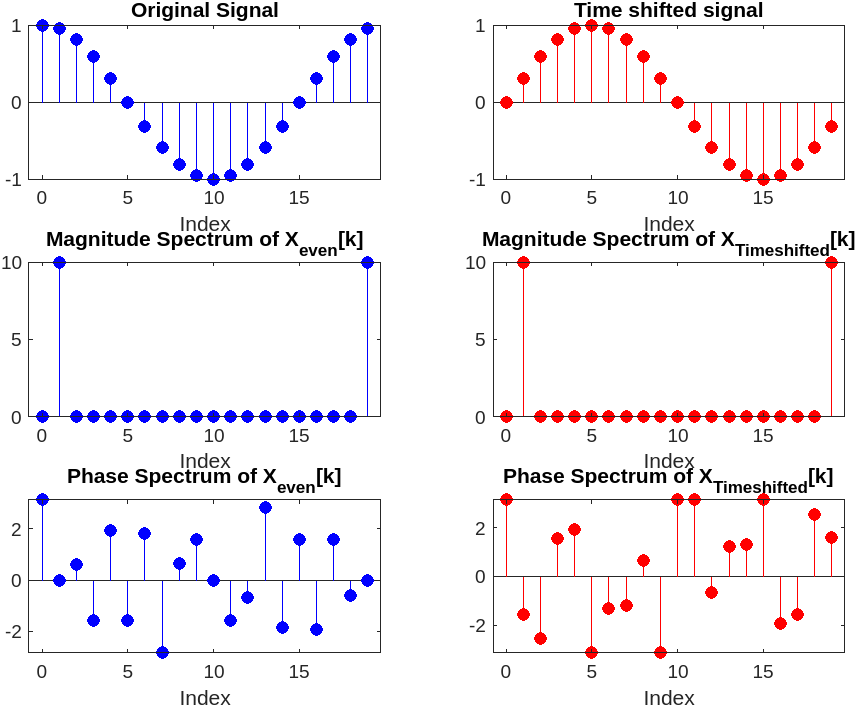
\includegraphics[width=0.8\textwidth]{DSP/eventimeshift.png}
    \caption{Matlab Plot for even signal timeshift,l=5.}
    \label{fig:example_image}
\end{figure}
\clearpage

Now for odd conjugate signal,
\[x_{\text{odd}}[n] &= j \sin\left(\frac{2\pi n}{20}\right) \\

\]
\begin{figure}[h]
    \centering
    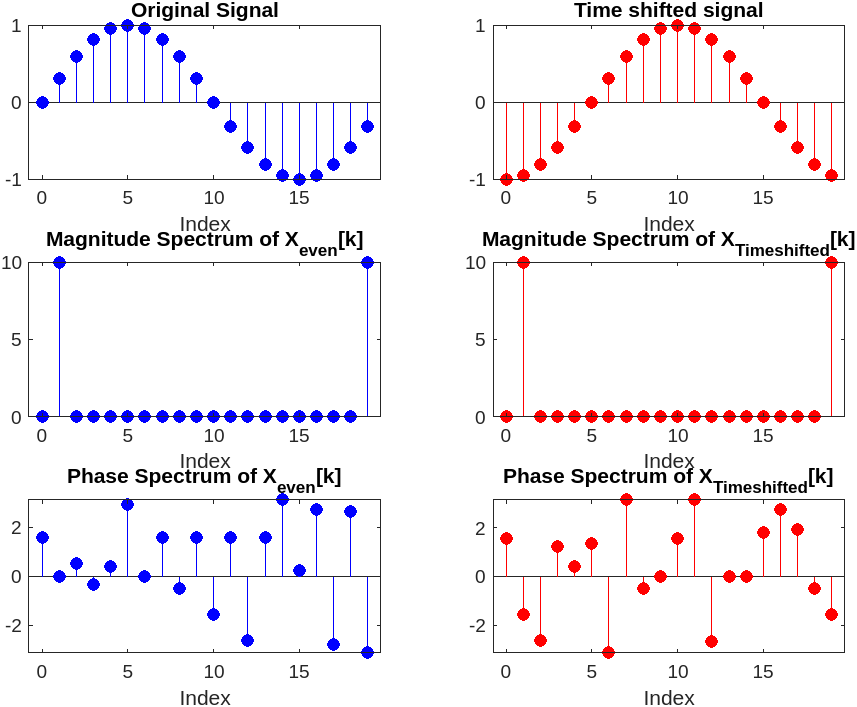
\includegraphics[width=0.8\linewidth]{DSP/oddtimeshift.png}
    \caption{Timeshift plot for Odd Conjugate Signal,l=5}
    \label{fig:enter-label}
\end{figure}

Now for a random signal
\begin{figure}[h]
    \centering
    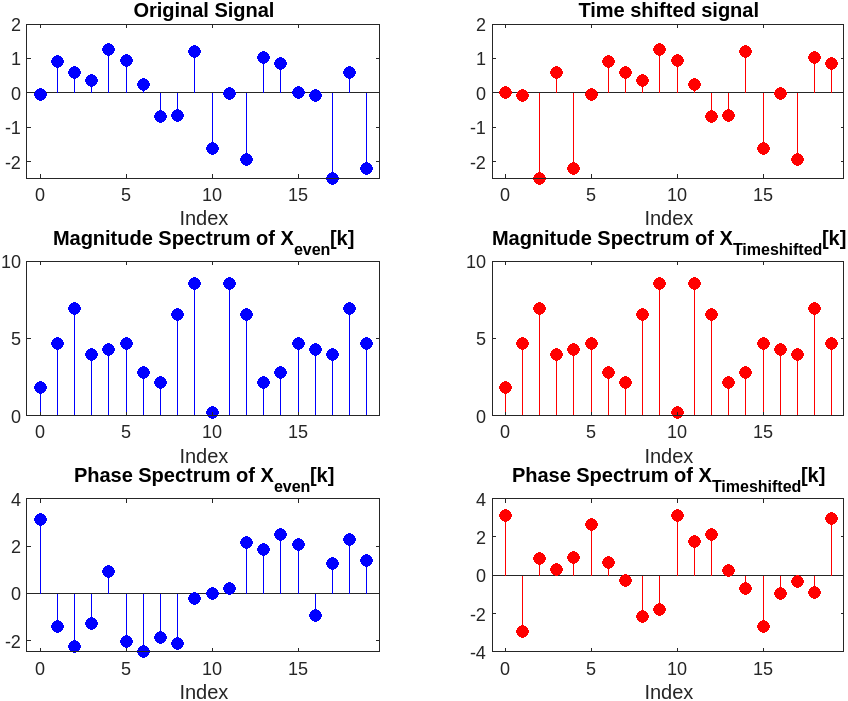
\includegraphics[width=0.8\linewidth]{DSP/Randomtimeshift.png}
    \caption{Timeshift Plot for a 20 pt random signal,l=5}
    \label{fig:enter-label}
\end{figure}
\clearpage

\section{Complex Conjugate}
The complex conjugate property of the Discrete Fourier Transform (DFT) states that 
\[
\mathcal{D}\left\{ x^*[n] \right\} = X^*[N - k]
\]

So For an Even real signal,
\[
 x_{\text{even}}[n] &= \cos\left(\frac{2\pi n}{20}\right)
\]
\begin{figure}[h]
    \centering
    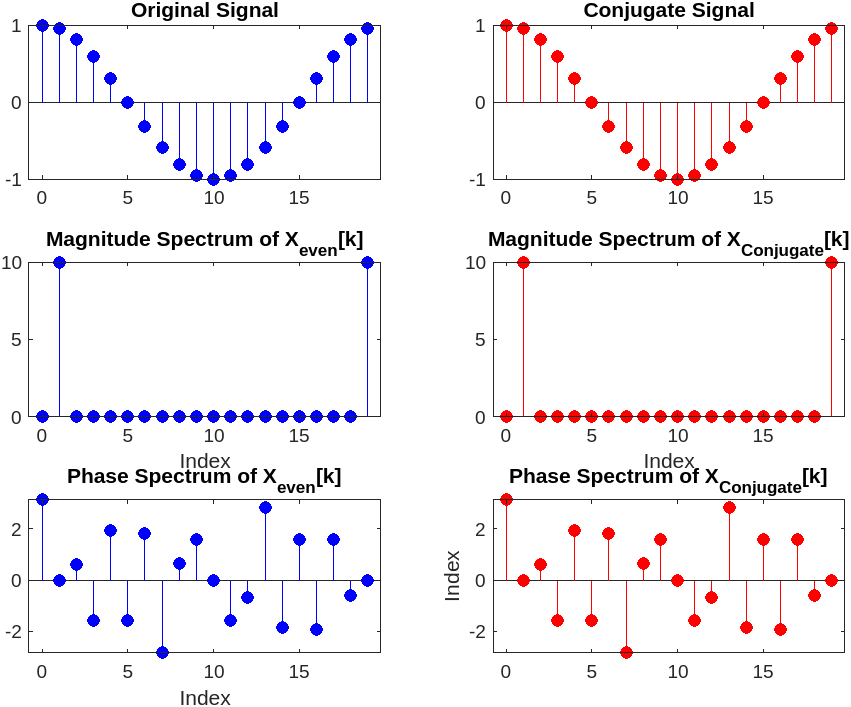
\includegraphics[width=0.8\textwidth]{DSP/evenconjugate.png}
    \caption{conjugate for even signal}
    \label{fig:enter-label}
\end{figure}

For an odd Conjugate Signal,
Now for odd conjugate signal,
\[x_{\text{odd}}[n] &= j \sin\left(\frac{2\pi n}{20}\right) \\

\]
\begin{figure}[h]
    \centering
    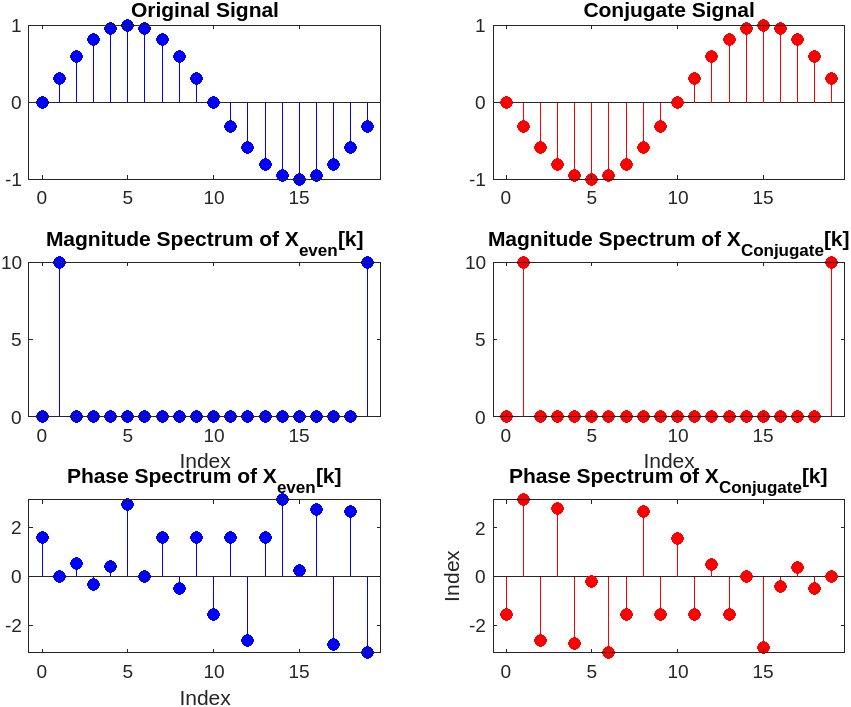
\includegraphics[width=0.8\textwidth]{DSP/oddconjugate.png}
    \caption{Conjugate Plot for odd Conjugate.}
    \label{fig:enter-label}
\end{figure}

\clearpage

And for a Random signal.
\begin{figure}[h]
    \centering
    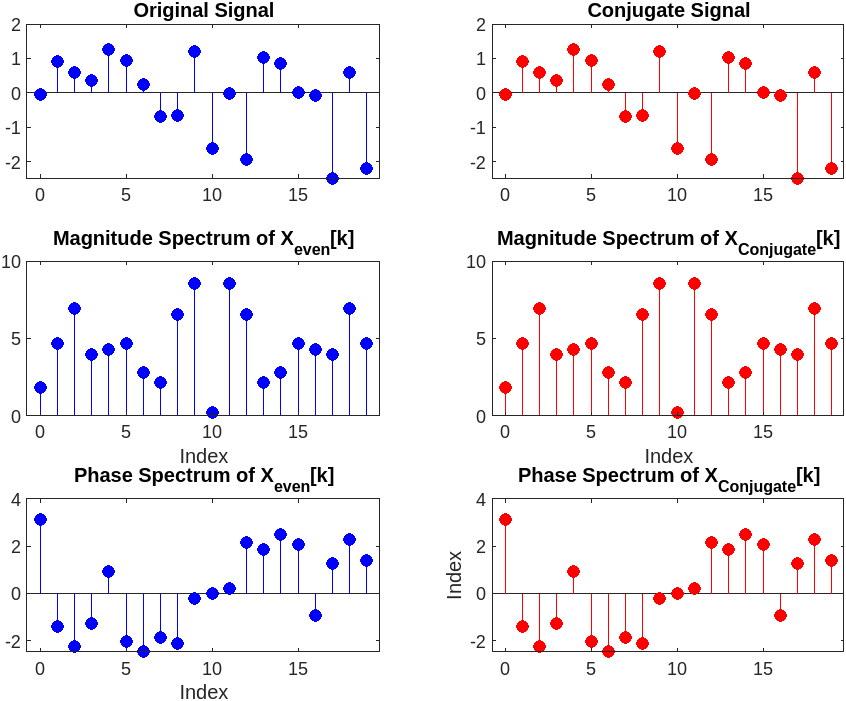
\includegraphics[width=0.8\textwidth]{DSP/Randomconjugate.png}
    \caption{Conjugate Plot for Random Signal.}
    \label{fig:enter-label}
\end{figure}


\section{Time Reversal Property of DFT}

The time reversal property ofDFT states that the DFT of a time-reversed signal is the complex conjugate of the DFT of the original signal, but with a reversal of the frequency indices
\[
\mathcal{D} \{ x[-n] \} = X^*[N - k]
\]

So For An Even real signal,
\[
 x_{\text{even}}[n] &= \cos\left(\frac{2\pi n}{20}\right)
\]
\begin{figure}[h]
    \centering
    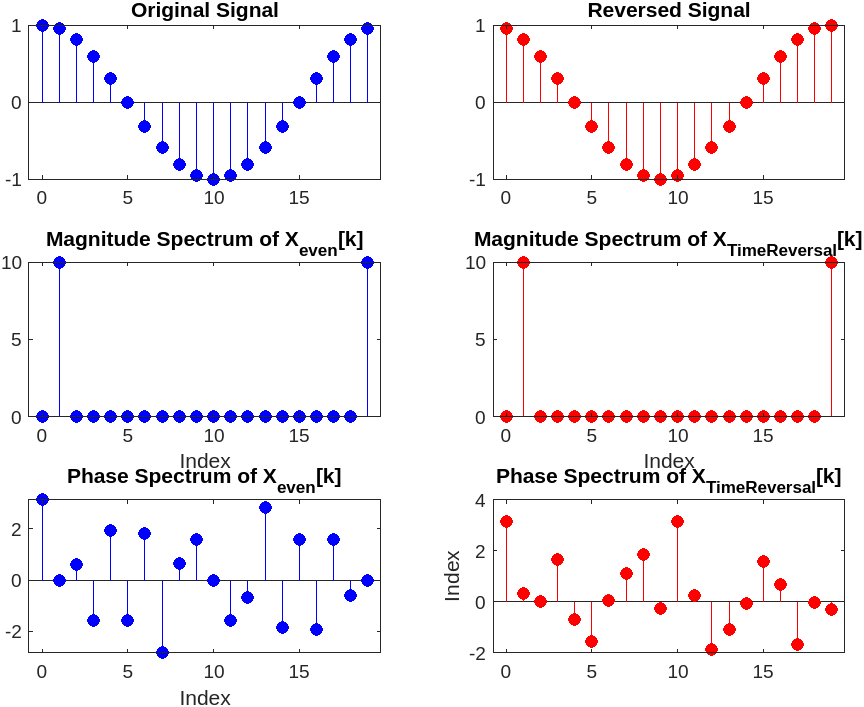
\includegraphics[width=0.8\linewidth]{DSP/evenreversal.png}
    \caption{Time Reversal Plot of Even signal.}
    \label{fig:enter-label}
\end{figure}
\clearpage

For an odd Conjugate Signal,
\[x_{\text{odd}}[n] &= j \sin\left(\frac{2\pi n}{20}\right) \\

\]
\begin{figure}[h]
    \centering
    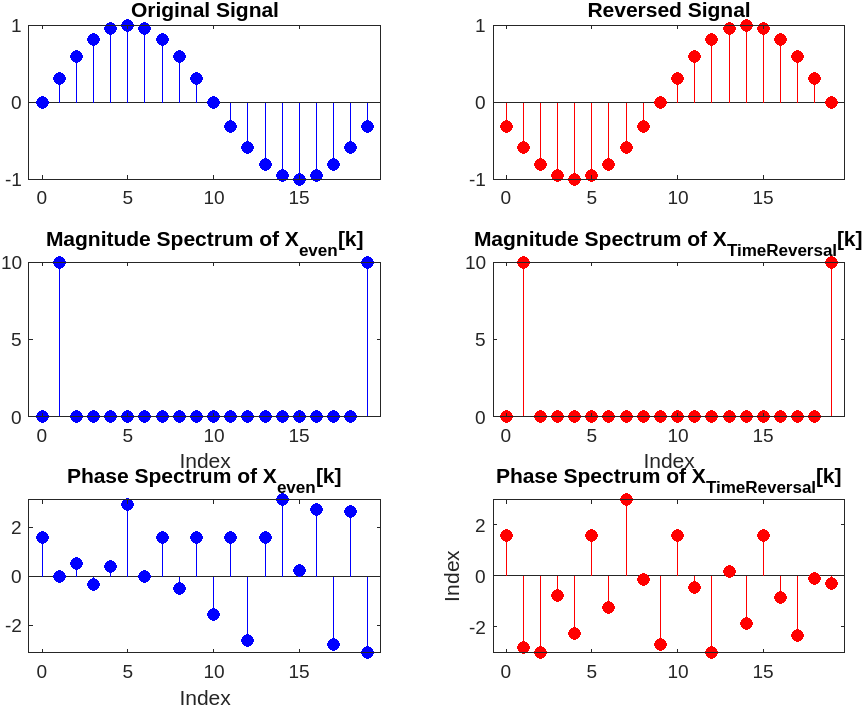
\includegraphics[width=0.8\textwidth]{DSP/oddtimereversal.png}
    \caption{Reversal Plot for odd Conjugate.}
    \label{fig:enter-label}
\end{figure}
\clearpage

For a random signal,
\begin{figure}[h]
    \centering
    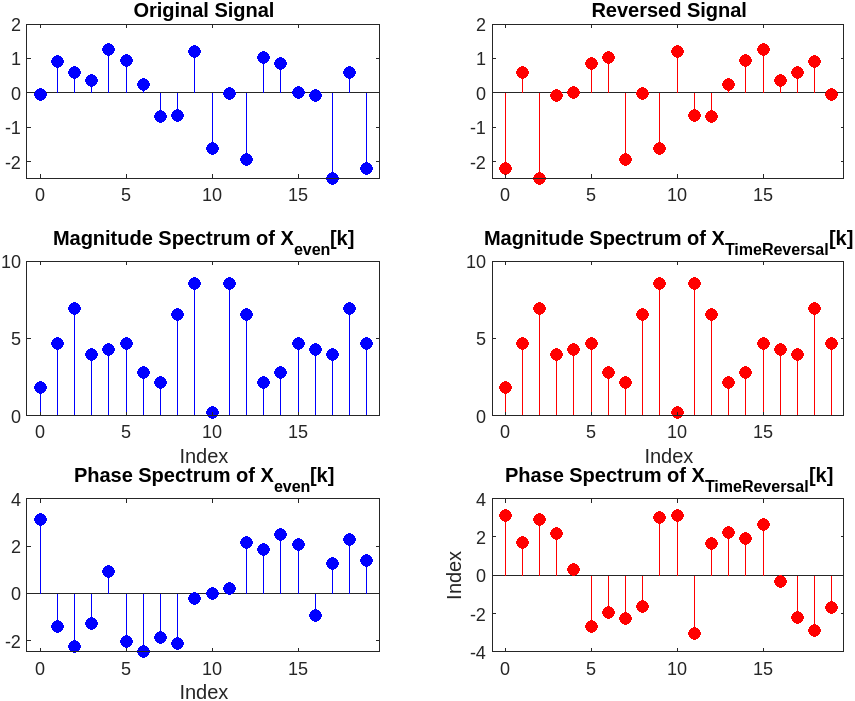
\includegraphics[width=0.8\linewidth]{DSP/Randomreverse.png}
    \caption{Reversal Plot for Random Signal}
    \label{fig:enter-label}
\end{figure}

\section{Frequency Shifts}
The frequency shift property states that multiplying a signal by a complex exponential in the time domain results in a shift in the frequency domain. 
\[
\mathcal{D}\left\{ x[n] e^{-j k_0 \frac{2\pi n}{N}} \right\} = X(k - k_0)
\]

So For An Even real signal,
\[
 x_{\text{even}}[n] &= \cos\left(\frac{2\pi n}{20}\right)
\]
\begin{figure}[h]
    \centering
    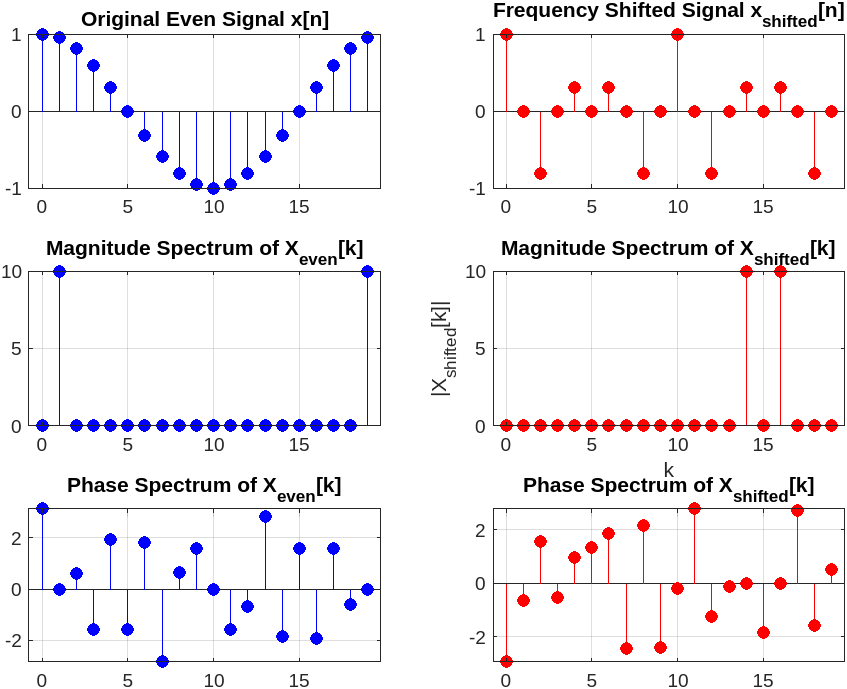
\includegraphics[width=0.8\linewidth]{DSP/evenfrequency.png}
    \caption{Frequency Shift Plot of Even signal.}
    \label{fig:enter-label}
\end{figure}
\clearpage

For an odd Conjugate Signal,
\[x_{\text{odd}}[n] &= j \sin\left(\frac{2\pi n}{20}\right) \\

\]
\begin{figure}[h]
    \centering
    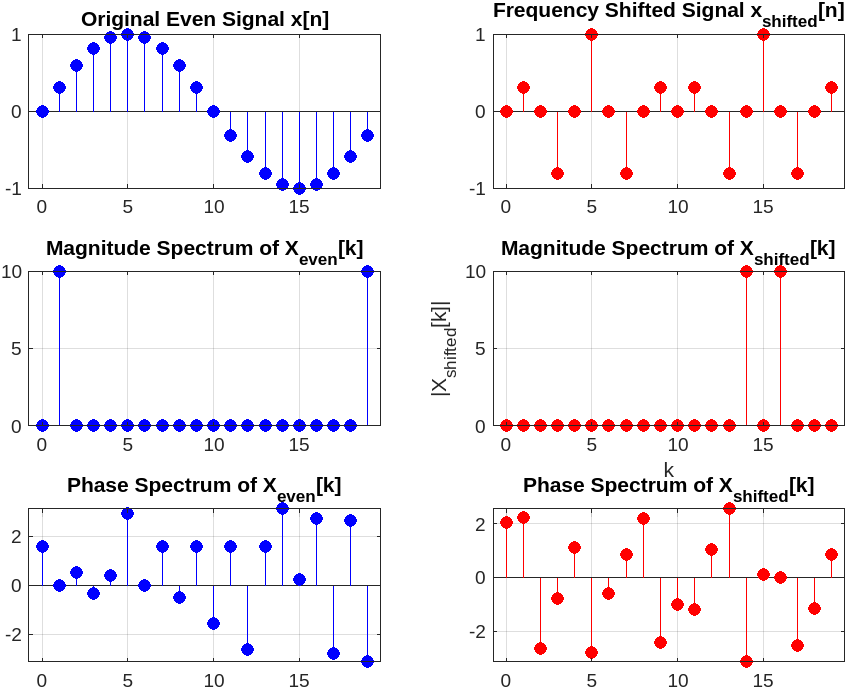
\includegraphics[width=0.8\textwidth]{DSP/oddfrequency.png}
    \caption{Frequency shift Plot for odd Conjugate.}
    \label{fig:enter-label}
\end{figure}

For a random signal,
\begin{figure}[h]
    \centering
    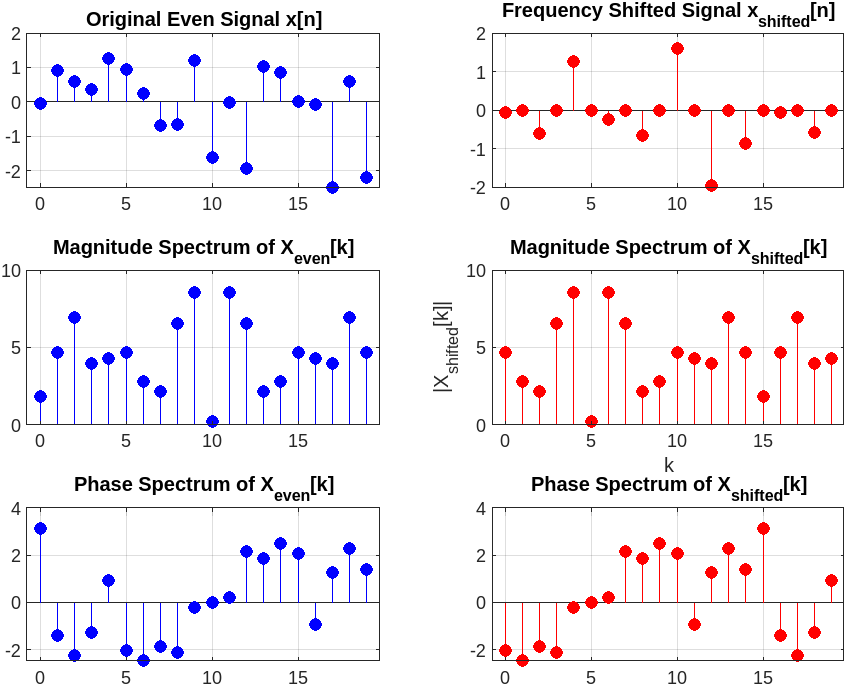
\includegraphics[width=0.8\linewidth]{DSP/Randomfrequency.png}
    \caption{Frequency shift Plot for Random Signal}
    \label{fig:enter-label}
\end{figure}
\end{document}



